%This is a experiment example of ZhengXiaoyang's experiment report template

\documentclass[UTF8]{ctexart}
 
\usepackage{amsmath}
\usepackage{cases}
\usepackage{cite}
\usepackage{xeCJK}
\usepackage{graphicx}
\usepackage[margin=1in]{geometry}
\geometry{a4paper}
\usepackage{fancyhdr}
\pagestyle{fancy}
\fancyhf{}

\graphicspath{{picture/}}


\title{刚体转动惯量测量}
\graphicspath{{picture/}}


\title{刚体转动惯量测量预习报告}
\author{郑晓旸}
\date{\today}
\pagenumbering{arabic}

\begin{document}
%这里是文件的开头
\fancyhead[L]{郑晓旸}
\fancyhead[C]{转动惯量}
\fancyfoot[C]{\thepage}

\maketitle
\tableofcontents
\newpage

\section{实验目的}
    \begin{itemize}
        \item 通过实验加深对刚体运动定律的理解
        \item 学习两种测量刚体转动惯量的实验方法
        \item 练习用曲线拟合方法处理数据
    \end{itemize}

\section{实验仪器}
\begin{itemize}
    \item PASCO 转动及扭摆实验组件(包含支架、转动传感器、力传感器、铝盘、测试圆环、挂钩、砝码、金属丝等)
    \item 550 通用接口
    \item Capstone 软件
    \item 其它:水平尺,螺旋测微计,游标卡尺,钢卷尺,电子天平等
\end{itemize}

\section{实验原理}

    \subsection{转动定律法}
    
    如图\ref{fig:2}所示,在转动惯量测量仪上,待测物体受到重力提供的外力矩$T$和摩擦力矩$T_\mu$的作用,根据转动定律有:
    \begin{equation}
    T-T_\mu=I\beta \label{eq:5}
    \end{equation}
    其中$I$为待测物体与转动惯量测量仪的总转动惯量,$\beta$为角加速度。外力矩大小为
    \begin{equation}
    T=mgr_0 \label{eq:6}
    \end{equation}
    其中$m$为砝码的质量,$g$为重力加速度,$r_0$为滑轮半径。
    
    在一系列不同重物作用下测得角加速度$\beta_i$,绘制$T$-$\beta$图像,如图\ref{fig:3}所示。图像应为一条斜率为$I$,截距为$-T_\mu$的直线。用最小二乘法拟合数据点,可得到总转动惯量$I$和摩擦力矩$T_\mu$。
    
    分别测量空载和负载两种情况下的总转动惯量$I_1$和$I_2$,两者之差即为待测物体的转动惯量:
    \begin{equation}
    I=I_2-I_1 \label{eq:7}  
    \end{equation}
    
    需要注意的是,由于摩擦力矩可能随转速变化,上述方法假设了$T_\mu$为常数。为尽量减小误差,应控制转速在较小的范围内变化。
    
    \begin{figure}[htbp]
    \centering
    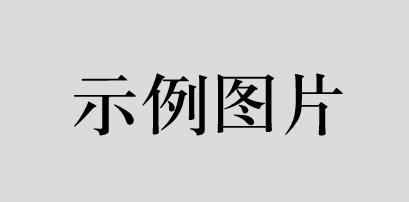
\includegraphics[width=0.6\textwidth]{rotating_platform.png}
    \caption{转动惯量测量仪受力分析} \label{fig:2}
    \end{figure}
    
    \begin{figure}[htbp]
    \centering
    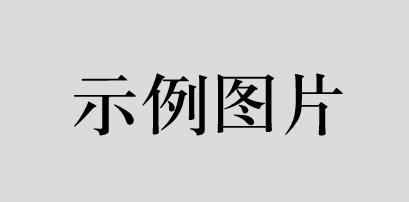
\includegraphics[width=0.6\textwidth]{T-beta.png}  
    \caption{外力矩$T$与角加速度$\beta$的关系} \label{fig:3}
    \end{figure}
    
    \subsection{扭摆法}
    
    如图\ref{fig:1}所示,将待测物体悬挂在扭丝上,偏离平衡位置后释放,在扭力矩$T$的作用下做扭摆运动。设转角为$\theta$,扭丝的扭力系数为$k$,则根据胡克定律有:
    \begin{equation}
    T=-k\theta \label{eq:8}
    \end{equation}
    由转动定律可得扭摆的运动方程为:
    \begin{equation}
    I\ddot{\theta}=-k\theta \label{eq:9}
    \end{equation}
    其中$I$为待测物体与扭摆的总转动惯量。这是一个简谐振动方程,特征角频率为
    \begin{equation}
    \omega=\sqrt{\frac{k}{I}} \label{eq:10}  
    \end{equation}
    
    实验中,先测量扭力系数$k$。在扭丝上施加一系列转角$\theta_i$,测量相应的回复力矩$T_i$,绘制$T$-$\theta$图像,如图\ref{fig:4}所示。图像应为一条过原点的直线,斜率即为$k$。
    
    然后测量扭摆周期$T$,由公式
    \begin{equation}
    \omega=\frac{2\pi}{T} \label{eq:11}
    \end{equation}
    计算特征角频率,代入公式(\ref{eq:10})即可求得总转动惯量:
    \begin{equation}
    I=\frac{kT^2}{4\pi^2} \label{eq:12}
    \end{equation}
    
    分别测量空载和负载两种情况下的扭摆周期,计算总转动惯量$I_1$和$I_2$,两者之差即为待测物体的转动惯量:
    \begin{equation}
    I=I_2-I_1 \label{eq:13}
    \end{equation}
    
    \begin{figure}[htbp]
    \centering
    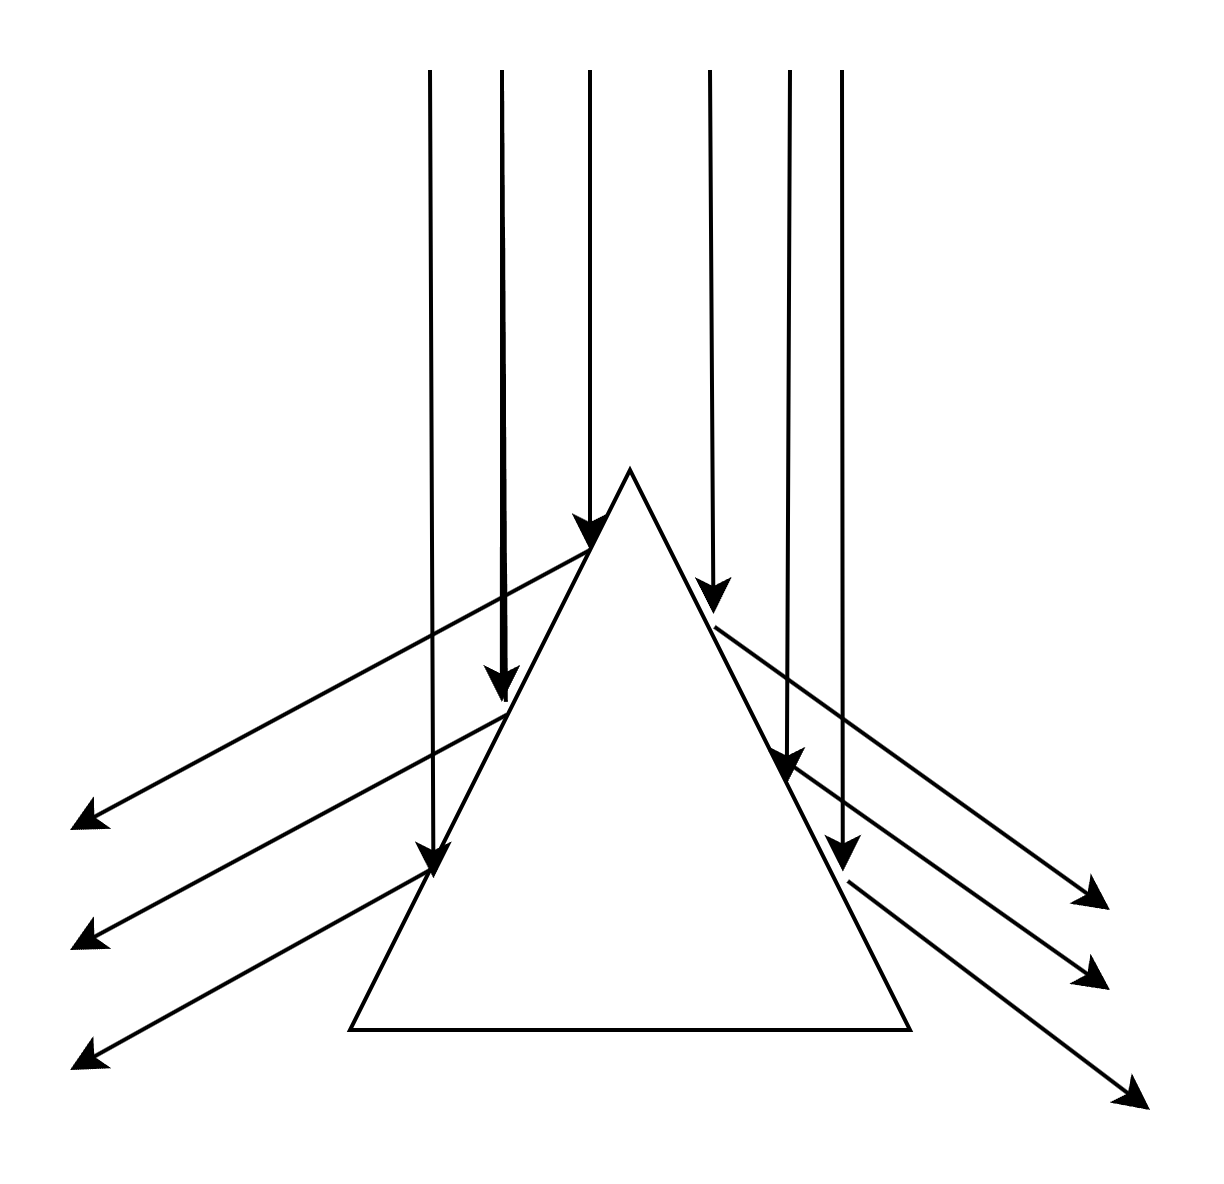
\includegraphics[width=0.6\textwidth]{T-theta.png}
    \caption{回复力矩$T$与转角$\theta$的关系} \label{fig:4}
    \end{figure}
    
    需要注意的是,由于存在空气阻力等因素,扭摆并非理想的无阻尼简谐振动,实际测得的周期会略大于理论值。为尽量减小误差,应使扭摆的初始振幅较小,并尽快测量周期。


\section{实验过程和数据分析}

\section{分析与讨论}

\subsection{误差分析}

\subsubsection{实验中的系统误差}


\subsubsection{实验中的偶然误差}
接线时可能有xxx情况,导致xxx。xx上的xx在某情况下有xx的问题存在,经反复调整后得以正常测量。

\subsection{实验后的思考}
可说明自己做本实验的总结、收获和体会,对实验中发现的问题提出自己的建议。

\newpage
%图一般很大,建议换页。



\end{document}
